\section{DataSet}
\label{sec:dataset}
We apply our approach to Stack Overflow (SO) and GitHub. We use code snippets in SO as the pool of user-input queries and use Java projects in GitHub as our code corpus to search from. We choose these two datasets not only because of their popularity within the programming community, but also because they are part of a larger system of software production. The same users that rely on the hosting and management characteristics of GitHub often have difficulties and need help on the implementation of their computer programs, seek support on SO for their specific problems, or hints of solutions from ones with a degree of similarity, and return to GitHub to apply the knowledge acquired. 

Previous work have shown that developers often copy and paste code snippets from Stack Overflow to their GitHub projects and make adaptations as needed~\cite{yang2017stack, an2017stack, wu2018developers, zhang2019analyzing}. Our approach will facilitate such opportunistic code reuse process when developers browse code snippets in SO. The use scenario will be: when a user is interested in a code snippet in SO, {\tool} recommends related code fragments from GitHub, showing what other code they may also want to investigate and integrate into their own project. 


\subsection{GitHub}
We downloaded Java projects on GitHub by querying GHTorrent~\cite{gousios2012ghtorrent}. GHTorrent is a scalable, offline mirror of data offered through the GitHub REST API, available to the research community as a service. It provides access to all the metadata of GitHub projects, e.g., the clone url, the number of stars and committers, main programming languages in a project, etc. We use these metadata to screen the projects. Our project selection criteria are:
\begin{itemize}
	\item We only consider GitHub projects that have at least five stars, in order to avoid toy projects that do not adequately reflect software engineering practices~\cite{kalliamvakou2014promises}.
	\item We only keep non-forked projects, because project forking leads to many identical projects and would unnecessarily skew our recommendation.
	\item Prior work on GitHub cloning finds many identical files among GitHub projects, since developers may copy the whole file into another project without making any changes~\cite{lopes2017dejavu}. To account for this internal duplication in GitHub, we remove duplicated GitHub files using the same file hashing method as in~\cite{lopes2017dejavu}.
\end{itemize} 

As a result, we downloaded 50,826 non-forked Java repositories with at least five stars from GitHub. After de-duplication, 5,825,727 distinct Java files remain.


\subsection{Stack Overflow}
We downloaded the SO dump taken in October 2016~\cite{stackexchange}. From the data dump, we extract code snippets in the markdown {\ttt <code>} from SO posts with {\ttt java} or {\ttt android} tags.
We consider code snippets in answer posts only, since snippets in question posts are rarely used as valid code examples. This results in 312,219 Java and Android answer posts.

Since SO snippets are often free-standing statements with low parsable rates~\cite{yang2016query}, we used a customized pre-processor before tokenization. For free-standing statements, we wraps them with dummy class and method definitions, and add semicolons after statements as needed. For snippets contain multiple methods, we chunk them into individual ones. We keep only parsable SO snippets after pre-processing.

Prior work finds that larger SO snippets have more meaningful clones in GitHub~\cite{yang2017stack}. Hence, we choose to study SO snippets with no less than 50 tokens after tokenization. We also remove duplicated examples within SO. As a result, we collect 186,392 distinct SO snippets.

\subsection{Result for similar code detection}
We run SoucererCC to find all similar pairs between SO and GitHub. We run on a server machine with 116 cores and 256G RAM. It takes 24 hours to complete. As a result, we get 21,207 distinct SO methods that have one or more similar code fragments in GitHub. We take these 21,207 SO snippets as our query code base.

\subsection{Quantitative analysis}
\todo{merge Figure 2,3,4 into one line}
We use 21,207 SO snippets as our query code base and get their similar counterparts in GitHub. 
The SO snippets have a median of two GitHub clones and a mean of one GitHub clones. The distribution of number of GitHub clones is shown in Figure \ref{fig:num-clone}. From the distribution we can see that SO snippets most commonly have zero to five similar counterparts in GitHub. Most of the SO snippets have less than twenty GitHub clones.

\begin{figure}
	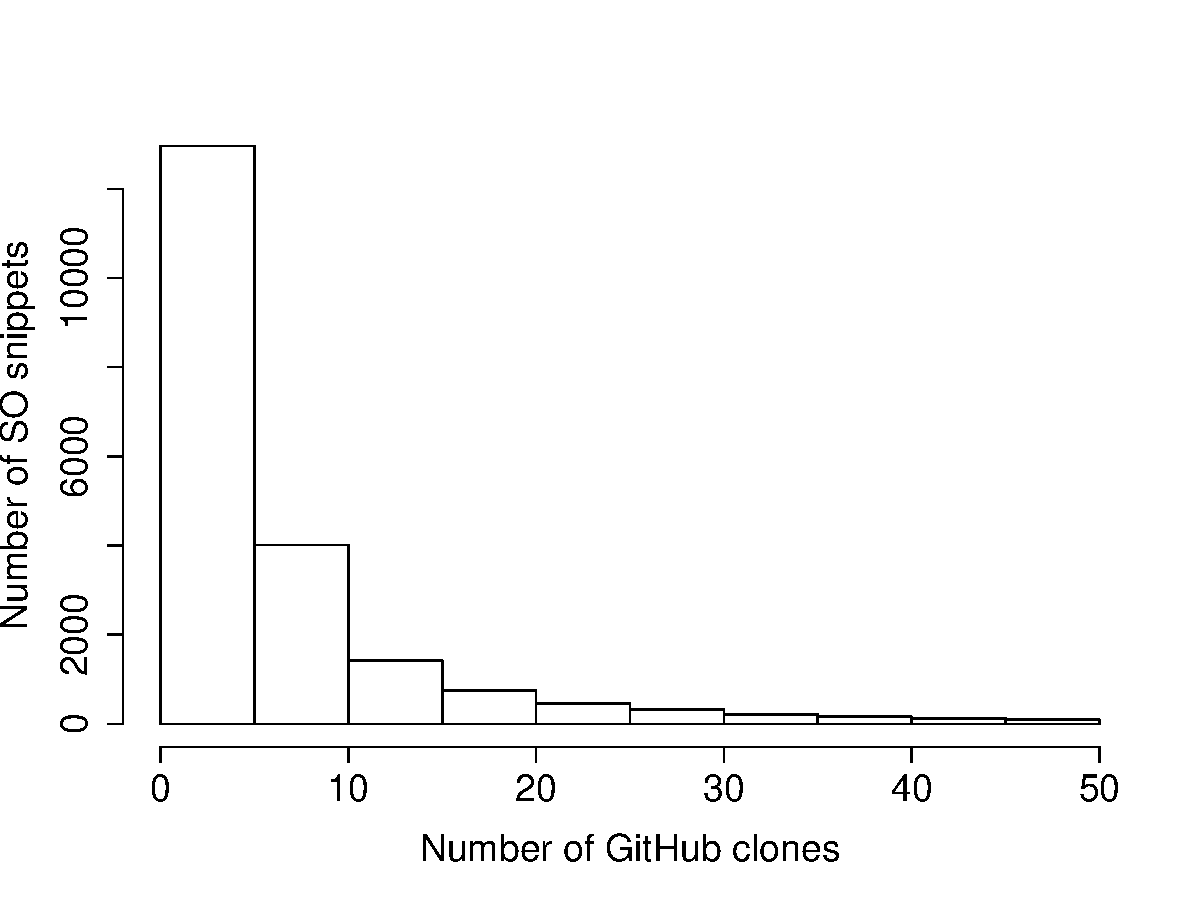
\includegraphics[scale=0.4]{figures/dist-gh-clone.pdf}
	\caption{Distribution of number of GitHub clones}
	\label{fig:num-clone}
\end{figure}

We collect the original GitHub files which contain these similar counterparts Then we extract all co-occurred methods from these GitHub files and treat them as candidate code fragments. For each candidate in each GitHub file, we cluster its similar counterparts from other files. We keep only the clusters with size of at least two and return the remaining clusters in descending order of size.

For 11,110 out of 21K SO queries, {\tool} can retrieve related code fragments from GitHub. That is, using our SO query code base and GitHub search code corpus, {\tool} can find common co-occurring code for 52.4\% of the queries. The SO queries have a median of 24 common co-occurring methods in GitHub and a mean of 74 common co-occurring methods. The retrieved methods have a median of 12 average lines of code, and a mean of 14 average lines of code. The distribution of number of related methods and distribution of average lines of code are shown in Figure \ref{fig:num-related} and \ref{fig:avg-loc} respectively.

From the figures we can see that a SO query most commonly have less than ten common co-occurring code fragments, and most of the SO queries have less than 50 common co-occurring methods in GitHub. Most related methods for a query will have five to thirty average lines of code.

\begin{figure}
	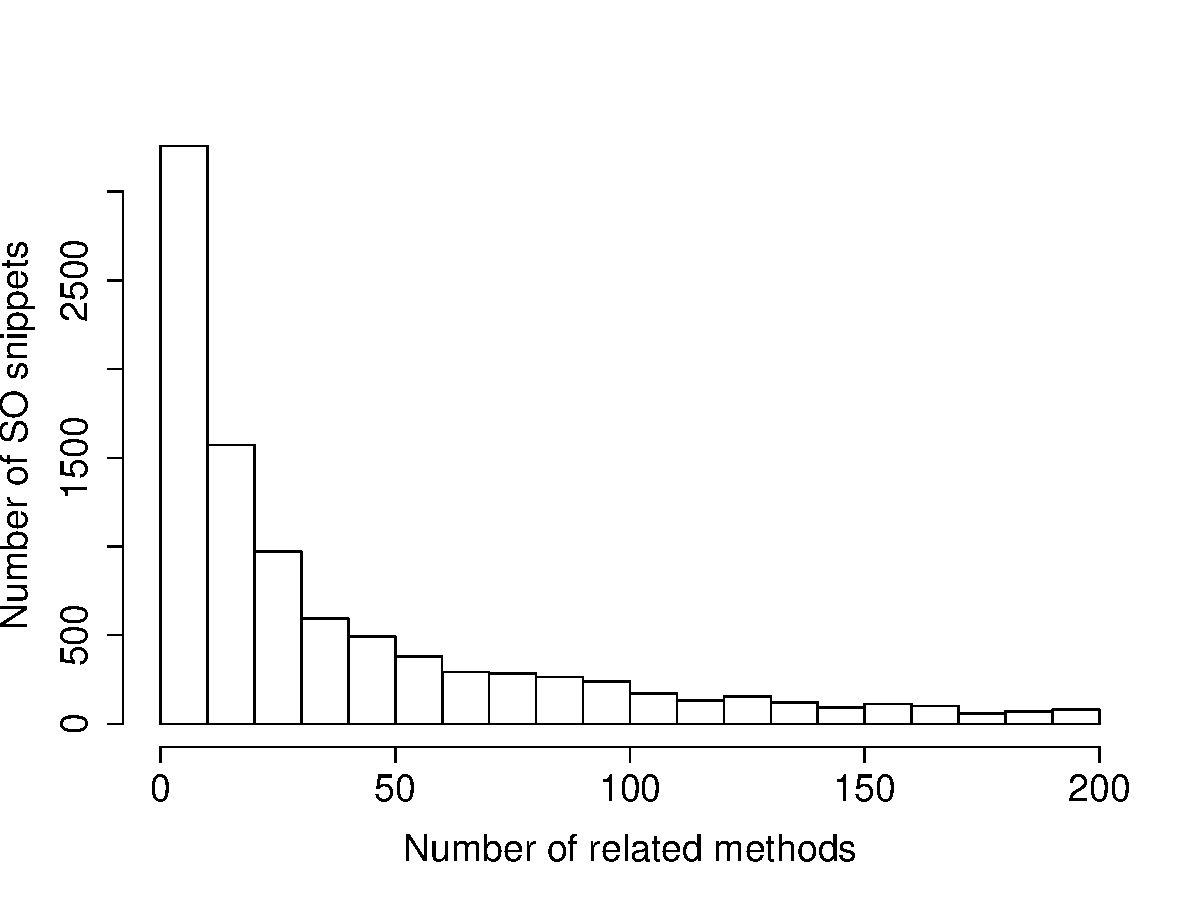
\includegraphics[scale=0.4]{figures/dist-related.pdf}
	\caption{Distribution of number of related methods}
	\label{fig:num-related}
\end{figure}

\begin{figure}
	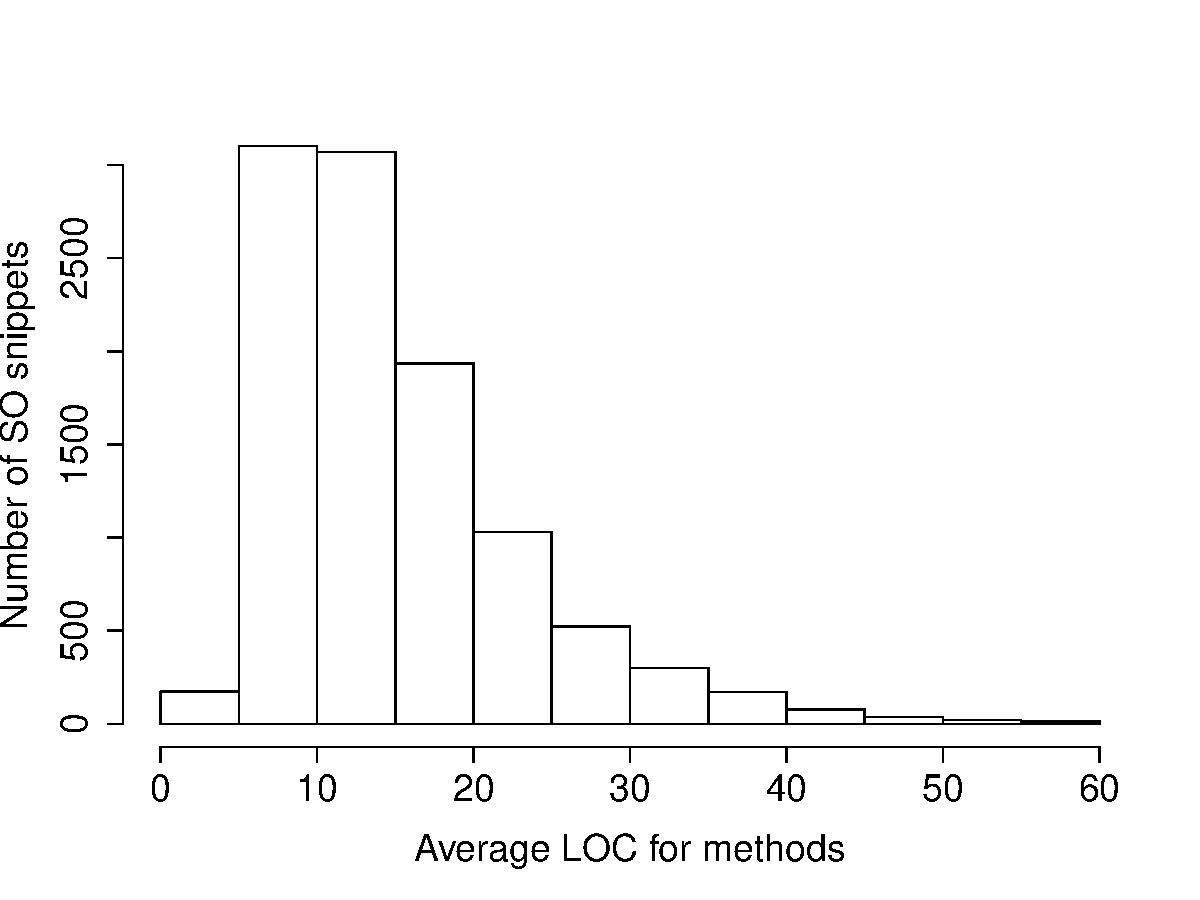
\includegraphics[scale=0.4]{figures/dist-loc.pdf}
	\caption{Distribution of average LOC of related methods}
	\label{fig:avg-loc}
\end{figure}

